\documentclass{article}

\PassOptionsToPackage{numbers,sort&compress}{natbib}
\usepackage[dblblindworkshop,final]{neurips_2026}
\workshoptitle{SLMs for Agentic Systems, Paris, France, 2026}

\usepackage[utf8]{inputenc}
\usepackage[T1]{fontenc}
\usepackage{float}
\usepackage[hidelinks]{hyperref}
\usepackage{url}
\usepackage{booktabs}
\usepackage{graphicx}
\usepackage{microtype}
\usepackage{xcolor}
\usepackage{amsmath}
\usepackage{multirow}

\title{Small Models, Exact Memories: Stress-Testing Optical Memory for Small Multimodal Agents}

\author{G{\"o}ktu{\u{g}} Aslano{\u{g}}lu\\Independent Researcher
  \And Viswanadh Vadlamani\\Safe App
  \And \c{S}uayp Talha Kocabay\\Independent Researcher}
\hypersetup{pdftitle={Small Models, Exact Memories: Stress-Testing Optical Memory for Small Multimodal Agents},pdfauthor={Goktug Aslanoglu, Viswanadh Vadlamani, Suayp Talha Kocabay}}

\begin{document}
\raggedbottom

\maketitle

\begin{abstract}
Can unmodified small multimodal readers use rendered histories as memory without losing exact state? We evaluate zero-shot optical memory through an 18-episode controlled stress test and long-horizon conversational QA. On a frozen 100-question LoCoMo subset, dense 8 px histories score .027/.099 F1 for Qwen3.5-2B/9B, versus .384/.410 for raw text and .415/.422 for input-count-matched BM25. Gold-selected evidence at the same density recovers to .383/.510; GLM-4.6V-Flash reproduces the qualitative pattern. Unreadability alone therefore cannot explain full-history failure, although selection, distractors, page count, and context use remain jointly implicated. A separate 500-question follow-up finds that BM25-selected optical evidence improves over full optical for all three readers, but the same evidence scores higher as text. In the controlled pilot, exact match at the only processor-measured compressed point spans 5.6\%--55.6\% across Qwen sizes; GLM reaches 27.8\%. A separate held-out identifier diagnostic improves exact recovery through layout changes at matched native input counts, without closing the gap to text. These results characterize a failure regime for naive dense optical packing, not a universal scaling law or a general disadvantage for engineered optical memory.
\end{abstract}

\section{Introduction}

Small-model agents accumulate dialogue, tool outputs, configuration values, identifiers, paths, and decisions under tighter memory and compute budgets than frontier systems. Keeping complete text histories is simple, while retrieval and summarization risk discarding an exact value before a later query is known. A complementary idea is to render history as visual pages and let a native multimodal model read them when needed. By \emph{exact state}, we mean later-needed values whose correctness is literal rather than semantic, such as hashes, paths, ports, configuration values, identifiers, and tool outputs.

Visual text is a credible representation: pixel and screenshot pretraining can recover linguistic structure \citep{rust2023pixel,lee2023pix2struct}, and off-the-shelf multimodal models sometimes replace text with fewer visual tokens \citep{li2025textpixels}. Purpose-built systems extend this approach through training, caching, retrieval, adaptive layout, or locate-and-transcribe interfaces \citep{cheng2026glyph,feng2026agentocr,li2026ocrmemory,liang2026vizomem,shi2026memocr}. Those successes do not establish that an unmodified small reader can reliably use dense rendered history. Long-document benchmarks instead predict separate bottlenecks in recognition, localization, retrieval, and reasoning \citep{ma2024mmlongbench,fu2025ocrbench,tu2026fico}.

We use \emph{small reader} operationally for the tested 0.8B--9B native multimodal checkpoints, not as a universal parameter threshold for SLMs. \emph{Zero-shot} means no optical-memory-specific reader training or fine-tuning. The original renderings are not optimized; a separate diagnostic selects a source-preserving layout before held-out evaluation. We evaluate memory representation and reading rather than end-to-end agent success: exact recall need not imply a correct tool call, plan, or downstream action. The title uses exact state as a stress-test axis, not as a claim of a universal semantic-versus-exact hierarchy.

We contribute a reproducible stress-test protocol combining exact-state probes, processor-specific input accounting, matched retrieval text, and selected-evidence diagnostics. The original study contains a controlled Qwen size sweep and a LoCoMo-100 comparison with a GLM second-family check. Separate follow-ups test query-time retrieve-then-render memory, exact-string layout sensitivity at matched input counts, and a longer generation cap. Each retains its own sample, interface, and analysis. We propose no new compression architecture and infer neither a universal scaling law nor compute savings from visual-token counts.

\section{Related work}

Long-context benchmarks distinguish nominal context length from effective retrieval and reasoning ability \citep{bai2024longbench,hsieh2024ruler}. LoCoMo is an LLM-generated and human-verified benchmark of single-hop, temporal, and multi-hop questions over multi-session conversations \citep{maharana2024locomo}; LongMemEval separates indexing, retrieval, and reading stages \citep{wu2025longmemeval}. We isolate representation and reading rather than evaluate a complete deployable memory architecture.

Existing optical-memory systems primarily ask how to make visual memory work through adaptation or engineered interfaces. AgentOCR trains optical self-compression; OCR-Memory combines retrieval with locate-and-transcribe access; MemOCR learns adaptive layout and budgeting; Fico broadly measures visual fidelity rather than diagnosing this agent-memory regime \citep{feng2026agentocr,li2026ocrmemory,shi2026memocr,tu2026fico}. Other work adds dedicated encoders, post-training, or visual-textual caching \citep{wei2025deepseekocr,cheng2026glyph,liang2026vizomem}, while matched textual baselines expose the gap between reconstruction and downstream utility \citep{lee2025bad}. Complementary GUI-agent work reports that full-image memory can reduce some state-level failures while increasing hidden-operation and grounding failures, and develops action-grounded crops with narrowed retrieval \citep{choi2026naive}; our setting instead studies rendered textual history, literal state, and zero-shot small-reader access. Relative to these lines, we jointly test exact-state probes, multi-page conversational memory, input-count-matched textual retrieval, and a second-family selected-evidence diagnostic.

\section{Study design}

\paragraph{Controlled pilot.}
We generate 18 synthetic agent histories averaging 7,152 Qwen text tokens. Six templates cover semantic decisions, numeric state, high-entropy identifiers, symbol paths, structured configuration, and code/tool state. Each has three early/middle/late target placements and nearby distractors. Every episode appears as raw text and as four uniform four-page renderings (nominal 12, 10, 8, and 6 px). For Qwen, these use 16,384, 11,236, 7,396, and 4,096 vision tokens, yielding source-to-vision ratios $C$ of .437, .637, .967, and 1.746. We call a condition compressed only when $C>1$; therefore 8 px is near parity and only 6 px achieves processor-measured input-count reduction. The templates probe literal recovery but are small and confounded by format, alphabet, and answer length.

\paragraph{External LoCoMo-100.}
With seed 20260826, we select ten conversations and, per conversation, five single-hop, three temporal, and two multi-hop questions (100 total). This frozen LoCoMo-100 subset is deterministic external evidence, not official full-benchmark performance. Raw histories already fit the tested native windows, so optical input is an alternative representation rather than context-length extension. The four-way diagnostic compares: full raw text; the complete conversation rendered at 8 px across 5.6 pages on average; gold-selected evidence rendered on one 8 px page; and turn-level BM25 text packed without exceeding each model's processor-reported full-optical input count. Qwen's full-history 8 px realization is compressed ($C=2.42$), unlike its controlled 8 px condition. The selected optical condition is deliberately diagnostic, not an efficiency baseline. Additional Qwen controls include source summaries, selected 24 px evidence, date-repaired temporal evidence, identical selected text, and question-only input.

\paragraph{Rendering.}
Controlled sources use black DejaVu Sans Mono text on white RGB pages, a 12 px source font, a 2,044-pixel square canvas, and 28-pixel margins. The smaller conditions preserve wrapping and page assignment, using LANCZOS resizing to 1,708, 1,372, and 1,036 pixels (rounded up to a 28-pixel grid). Actual glyph sizes are approximately 12, 10.03, 8.05, and 6.08 px. Font size therefore varies jointly with canvas size, visual-token count, and resampling. LoCoMo-100 uses native 8 px text on 1,372-pixel square pages with 24-pixel margins for both full and gold-selected optical evidence; these conditions differ in content and page count, not nominal font size.

\paragraph{Models, budgets, and inference.}
The controlled Qwen matrix evaluates Qwen3.5-0.8B, 2B, 4B, and 9B; external Qwen validation uses the 2B and 9B endpoints \citep{qwen2026qwen35}. GLM-4.6V-Flash supplies a second-family controlled matrix and four-way LoCoMo diagnostic \citep{zai2026glm46v}. All original runs use greedy BF16 inference on one NVIDIA A100-SXM4-40GB with seed 20260826. Controlled and LoCoMo generation caps are 64 and 96 tokens; a post-hoc short-answer sensitivity uses 32. Throughout, compression means processor-reported input-count reduction only. We do not equate text and visual tokens in FLOPs, memory traffic, latency, or energy, and ratios are interpreted only within each processor. GLM is never placed on the Qwen parameter regression. For example, GLM's controlled 12/10/8/6 px conditions use 21,316/14,884/9,604/5,476 visual tokens and $C=.320/.459/.711/1.247$.

Qwen chat templates explicitly request \texttt{enable\_thinking=False}, falling back to the native template if that argument is unsupported. Neither family receives optical-memory-specific adaptation. Appendix~\ref{app:resources} reports the available synchronized generation timings, not end-to-end memory-system latency.

\paragraph{Scoring and uncertainty.}
Controlled recall uses normalized exact match; LoCoMo uses its stemmed token F1. Answer normalization applies the same enclosing-wrapper removal to both families and preserves complete LoCoMo answers, including multiline lists (Appendix~\ref{app:scoring}). Archived generations are unchanged. Qwen uncertainty is clustered by episode or conversation. LoCoMo-100 contrasts use 50,000-replicate conversation-cluster bootstrap intervals and exact two-sided sign-flip tests over ten conversation effects. The smallest attainable two-sided $p$ value is $2/2^{10}=.001953$; repeated values at this floor do not distinguish effect sizes. Sign-flip inference assumes sign symmetry under the null, not randomized assignment. Nonsignificance is not equivalence.

\paragraph{Separate stress-test follow-ups.}
The retrieval study uses 500 questions from the same ten conversations, disjoint from LoCoMo-100. The layout diagnostic uses 12 development and 48 held-out identifier cases, not additional instances of the six pilot templates. Its primary tests are paired exact McNemar tests with Holm correction across three readers. The cap diagnostic extends only the 500-question study's capped Qwen outputs. Appendices~\ref{app:followup}--\ref{app:cap} give the frozen protocols; no follow-up is pooled with the original study.

\section{Results}

\subsection{Dense multi-page optical memory fails against matched textual retrieval}

\begin{figure}[!htbp]
  \centering
  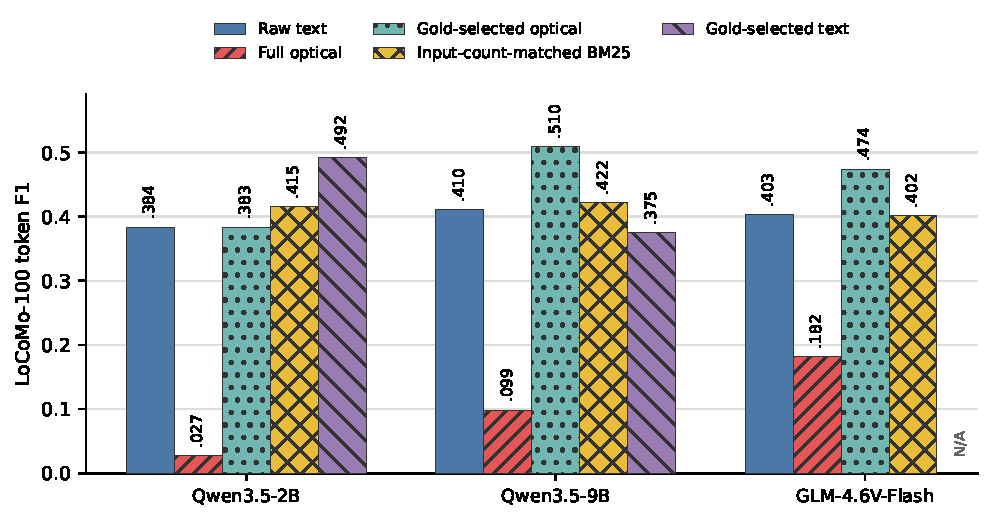
\includegraphics[width=\linewidth]{figures/figure_1_locomo_cross_family.pdf}
  \caption{LoCoMo token F1 on the frozen LoCoMo-100 subset. Gold-selected optical and identical selected text are diagnostics; GLM selected text was not run. BM25 is input-count-matched to full optical within each processor; text and visual counts are not assumed compute-equivalent.}
  \label{fig:locomo}
\end{figure}

Figure~\ref{fig:locomo} compares the conversational-memory conditions, including the selected-text control; exact values are tabulated in Appendix Table~\ref{tab:locomo}. Qwen full 8 px history achieves a 2.42x processor-reported count ratio (25,067 source tokens to 10,354 vision tokens) but scores only .027/.099 F1 at 2B/9B, versus .384/.410 from raw text. Input-count-matched BM25 reaches .415/.422. In paired conversation inference, BM25 exceeds full optical by +.388 at 2B (95\% CI [.317,.463], $p=.00195$) and +.324 at 9B ([.239,.409], $p=.00195$). Raw-minus-BM25 contrasts do not reject zero; this is not evidence of equivalence with ten conversation clusters.

GLM provides a second-family qualitative replication with its own processor counts. Full optical averages 13,446 vision tokens for 23,623 source tokens ($C=1.75$), while BM25 packs 13,435 text tokens. Full optical scores .182 F1, compared with .403 raw and .402 BM25. Raw-minus-full is +.221 (conversation-cluster bootstrap CI [.154,.284]) and BM25-minus-full is +.219 [.156,.289], both with exact sign-flip $p=.00195$. This is a shared failure pattern, not evidence for a universal law or directly comparable cross-processor token scale.

\subsection{Selected evidence diagnoses a combined context-use bottleneck}

Gold-selected evidence rendered at the same 8 px density raises Qwen F1 from .027 to .383 and from .099 to .510. For GLM, selected optical reaches .474; selected-minus-full is +.292 (CI [.213,.370], $p=.00195$), and every conversation effect is positive. The strong selected-optical result rules out simple 8 px unreadability as a sufficient explanation for full-history failure.

The intervention does not identify selection alone: it jointly changes evidence selection, distractor load, page count, and context structure. Selected 8 px occupies one page and is intentionally diagnostic rather than efficient; 111 Qwen text tokens become 1,849 visual tokens on average. Identical selected evidence as text scores .492/.375, revealing checkpoint-specific interface behavior rather than visual superiority. Question-only F1 is .005 at both endpoints, ruling out a simple answer-prior account. Thus the shared result is a qualitative selection/context-use pattern, not a single identified cause.

\subsection{Controlled exact-state fidelity at the tested visual budgets}

All five readers answer all 18 raw controls correctly. Within Qwen3.5, optical aggregate accuracy rises from 44.4\% at 0.8B to 73.6\%, 81.9\%, and 84.7\%. An exploratory episode-clustered trend estimates +.114 accuracy per parameter doubling (95\% CI [.072,.157]), but most statistically resolved improvement occurs from 0.8B to 2B; GLM is not included in this scale analysis. At the only compressed Qwen point ($C=1.746$), exact match is 1/18, 7/18, 8/18, and 10/18. GLM falls from 17/18 at 12 px to 5/18 at its only compressed point ($C=1.247$). Figure~\ref{fig:frontier} and Table~\ref{tab:controlled} expose heterogeneous exact-state failures rather than one fidelity threshold.

\begin{figure}[!htbp]
  \centering
  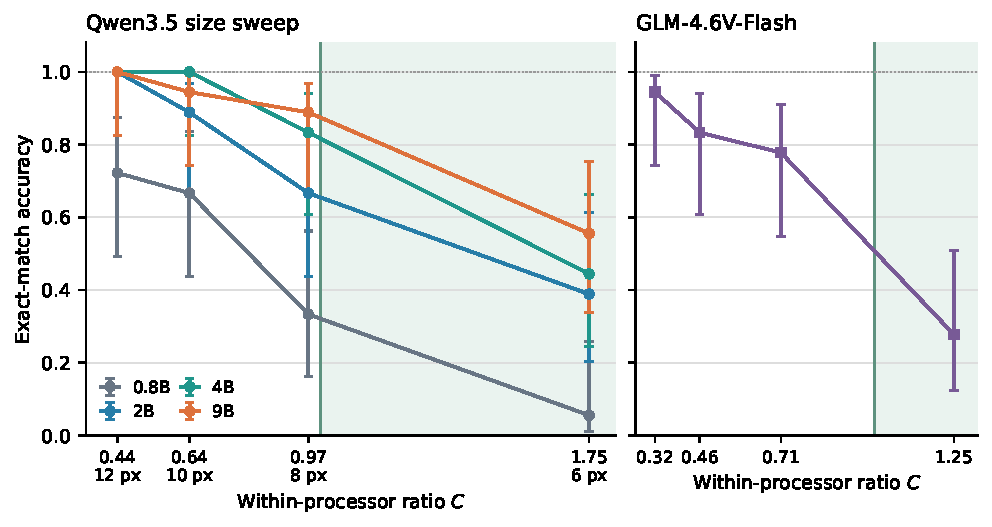
\includegraphics[width=\linewidth]{figures/figure_2_controlled.pdf}
  \caption{Controlled literal recall across tested optical budgets. Points run from nominal 12 to 10, 8, and 6 px left to right in each panel; all raw controls are 18/18. The shaded $C>1$ region denotes processor-measured input-count reduction, with only one tested point per family. Glyph size, canvas size, resampling, and input count covary; no isolated causal compression effect follows. Error bars are 95\% Wilson intervals over 18 episodes.}
  \label{fig:frontier}
\end{figure}

\begin{table}[H]
  \caption{Controlled exact matches out of 18 episodes per condition. GLM is a second-family check, not a point on the Qwen size curve.}
  \label{tab:controlled}
  \centering
  \small
  \begin{tabular}{lrrrrrr}
    \toprule
    Reader & Raw & 12 px & 10 px & 8 px & 6 px & Optical total \\
    \midrule
    Qwen3.5-0.8B & 18 & 13 & 12 & 6 & 1 & 32/72 \\
    Qwen3.5-2B   & 18 & 18 & 16 & 12 & 7 & 53/72 \\
    Qwen3.5-4B   & 18 & 18 & 18 & 15 & 8 & 59/72 \\
    Qwen3.5-9B   & 18 & 18 & 17 & 16 & 10 & 61/72 \\
    \midrule
    GLM-4.6V-Flash & 18 & 17 & 15 & 14 & 5 & 51/72 \\
    \bottomrule
  \end{tabular}
\end{table}

Descriptively, the tested exact-state templates do not share a single fidelity threshold. At Qwen3.5-9B, pooled counts across the four optical budgets are 12/12 for numeric state, 10/12 for high-entropy identifiers, 8/12 for symbol paths, 10/12 for structured configuration, and 9/12 for code/tool state. Semantic decisions are 12/12. Because each type-budget cell contains only three examples and templates differ in format and answer alphabet, these comparisons are diagnostic rather than causal.

\subsection{Exact-string layout sensitivity at matched input counts}
\label{sec:layout}

A separate diagnostic tests whether rendering geometry matters beyond measured input count. After one development round, we compare the original narrow layout with full-width word wrapping on 48 fresh held-out identifier cases. Both retain the same source on four pages at $C\approx2$ and have identical processor-native vision, nonvision, and total input counts, image grids, and input-ID sequences within each case and reader. Pixel tensors differ. This matches allocation, not the effective visual input.

\begin{table}[!htbp]
  \centering\small
  \caption{Separate identifier diagnostic: exact matches out of 48 held-out cases. The two $C\approx2$ layouts are input-count-matched; enlarged images and full text are larger-budget references. These cases are not pooled with the 18-episode pilot.}
  \label{tab:layout}
  \begin{tabular}{lrrr}
\toprule
Representation & Qwen2B & Qwen9B & GLM \\
\midrule
Full text & 47/48 & 46/48 & 48/48 \\
Original layout, $C\approx2$ & 0/48 & 0/48 & 0/48 \\
Full-width layout, $C\approx2$ & 6/48 & 21/48 & 7/48 \\
Enlarged-image reference & 17/48 & 35/48 & 29/48 \\
\bottomrule
\end{tabular}

\end{table}

Full-width wrapping raises exact recovery from 0/48 to 6/48, 21/48, and 7/48 for Qwen2B, Qwen9B, and GLM; all three paired differences remain statistically significant after Holm correction (Appendix~\ref{app:layout}). Recovery remains below text. The enlarged-image reference also fails the prespecified 36/48 success criterion for every reader. Thus native input count alone does not determine exact-state fidelity. Wrapping, whitespace, and pagination change jointly, so the result does not isolate glyph size or propose a new memory method.

\subsection{Deployable selection: a separate retrieval follow-up}
\label{sec:followup}

Gold evidence is not an available deployment input. A separately frozen retrieve-then-render study evaluates query-time selection on 500 additional questions from the same ten conversation clusters (105 multi-hop, 108 temporal, and 287 single-hop). Query-time BM25 selects the top 16 turns using only the question and conversation, then restores source order. Retrieved text and optical arms receive identical evidence strings and metadata; selected optical uses an 8 px, 1,372-pixel square page, while full optical is calibrated to $C\approx2$. Model/processor revisions are pinned, decoding is greedy BF16 with inference seed 2026090506 and a 96-token cap, and no reference answers or evidence annotations enter retrieval. This follow-up changes question coverage and source serialization; its conversation-macro F1 must not be pooled with LoCoMo-100. It adds coverage, not new independent conversations. Full protocol and paired intervals are in Appendix~\ref{app:followup}.

\begin{table}[H]
  \centering\small
  \caption{Separate 500-question follow-up, conversation-macro F1 over ten clusters. The two BM25-selected arms share evidence; the two budget-matched text arms may select different evidence.}
  \label{tab:followup}
  \begin{tabular}{lrrr}
\toprule
Representation & Qwen2B & Qwen9B & GLM \\
\midrule
Full text & .484 & .530 & .483 \\
Full optical ($C\approx2$) & .098 & .160 & .248 \\
BM25-selected text & .400 & .372 & .376 \\
BM25-selected optical, 8 px & .289 & .353 & .309 \\
Text at full-optical budget & .483 & .498 & .440 \\
Text at selected-optical budget & .407 & .391 & .393 \\
\bottomrule
\end{tabular}

\end{table}

Retrieved optical exceeds full optical by +.190 at Qwen2B (95\% cluster CI [.158,.225]), +.193 at Qwen9B ([.150,.230]), and +.060 at GLM ([.024,.095]). The same retrieved evidence as text nevertheless scores higher by .111, .019, and .067, respectively (paired intervals in Appendix~\ref{app:followup}). This supplies a deployable intermediate between full history and gold selection, without treating those different studies as a controlled oracle gap. Selection remains jointly coupled to page count, distractor load, and context structure; no component-level causal attribution follows.

\paragraph{Longer-generation sensitivity.}
Extending the cap from 96 to 256 tokens for the 126 Qwen2B and 121 Qwen9B capped full-optical outputs changes the reconstructed 500-question F1 from .0984 to .0999 and .1595 to .1610. Every original 96-token prefix is preserved. Both paired cluster intervals include zero, and 30 outputs still reach 256 tokens (Appendix~\ref{app:cap}). This bounded extension does not remove the retrieval advantage; it does not show that generation length never matters.

\section{Discussion and limitations}

\paragraph{Three diagnostic layers.}
The evidence distinguishes, without identifying independent causes, three layers. \emph{Recognition and layout:} selected 8 px pages are often readable, while the separate identifier test changes exact recovery at matched input counts. \emph{Selection and context use:} full LoCoMo adds pages, distractors, discourse structure, and evidence competition; selection changes these jointly. \emph{Output and reasoning:} temporal questions and generation behavior add failures beyond legibility. The bounded cap extension yields only small observed changes. These findings motivate retrieving before choosing a representation and retaining exact technical state symbolically when needed.

\paragraph{Relation to engineered optical memory.}
Our negative zero-shot result is compatible with engineered systems such as AgentOCR, OCR-Memory, MemOCR, and Glyph. They add learned or specialized memory interfaces beyond our fixed-reader stress tests. The layout diagnostic itself shows that rendering choices matter. We identify a dense multi-page failure regime, not that optical memory is generally ineffective.

\paragraph{Small controlled set and one-family size curve.}
The controlled pilot has 18 episodes and three examples per template; type is confounded with format, length, repetition, and distractor design, and development reused the pool. Glyph size, canvas size, resampling, and visual count change together, with only one compressed point. The separate 48-case identifier diagnostic does not enlarge this six-type pilot or identify a glyph-only effect. The Qwen size association may reflect training and optimization as well as size; GLM replicates a qualitative pattern, not a scale curve. Fixed-glyph budget manipulations, additional compressed pilot points, and graded distractors remain untested.

\paragraph{Subset, gold selection, and one external density.}
LoCoMo-100 has ten clusters with fixed 5/3/2 category quotas, omits open-domain and adversarial questions, and is not full-benchmark performance. Gold selection is diagnostic, changes several context properties, and is not deployable retrieval. The 500-question follow-up tests deployable selection but reuses the ten clusters and differs in serialization and question mix. Neither study includes a readable-density full-history control. Raw histories already fit native windows, and token-count reduction does not imply FLOPs, latency, energy, or memory-traffic savings.

\paragraph{Memory access rather than end-to-end agency.}
We measure recall and conversational QA, not whether recovered state produces a correct tool call, plan, or action. Temporal questions also expose reasoning and evidence-sufficiency limits beyond metadata and legibility.

\paragraph{Post-hoc output sensitivity and reproducibility.}
On LoCoMo-100, Qwen3.5-9B hits the 96-token cap on 42\% of full-optical questions. A post-hoc 32-token shortest-answer test does not rescue F1, but caps 84\% of 9B outputs and therefore does not isolate verbosity (Appendix~\ref{app:outputs}). The separate 500-question cap extension also leaves some outputs capped. These tests do not fully separate access, reasoning, and output compliance. Timings are single-pass A100 measurements without warm-ups, randomized repeats, or prefill/decode separation; no speed claim is made. Original Qwen runs omit exact revision hashes; the later diagnostics retain pinned snapshots. Seeded greedy CUDA inference is not guaranteed to be bitwise reproducible.

\paragraph{Ethics and deployment.}
Controlled histories are synthetic and LoCoMo is LLM-generated and human-verified; no private deployed-agent logs are used. Deployed long-term memory would still require consent, retention limits, access control, deletion, provenance, and representation-independent auditing.

\section{Conclusion}

Zero-shot optical memory is readable but not automatically usable as dense long-horizon memory. Within Qwen3.5, larger readers recover more exact state, yet the pilot's only processor-measured compressed condition remains unreliable. On frozen LoCoMo-100, full rendered histories underperform raw and input-count-matched retrieval text, while gold-selected evidence at the same density recovers strongly. GLM-4.6V-Flash shows the same qualitative pattern.

The separate retrieval follow-up supplies a deployable intermediate: retrieve-then-render improves over full optical, while same-evidence text remains better. The identifier diagnostic shows layout sensitivity at matched native counts; the longer cap does not remove the LoCoMo retrieval advantage. Together, these stress tests motivate selecting evidence before choosing a representation and retaining exact state through symbolic channels when needed. They establish neither a causal compression effect, a universal scaling law, nor a general disadvantage of optical memory.

\clearpage
\bibliographystyle{plainnat}
{\small\bibliography{references}}

\appendix

\section{Exact LoCoMo values}

\begin{table}[H]
  \caption{Exact values underlying Figure~\ref{fig:locomo}. Official LoCoMo token-F1 on the frozen LoCoMo-100 subset; the BM25 input count is matched to full optical within each processor.}
  \label{tab:locomo}
  \centering
  \small
  \begin{tabular}{lrrrrr}
\toprule
Reader & Raw & Full optical & Gold optical & BM25 & Gold text \\
\midrule
Qwen3.5-2B & .384 & .027 & .383 & .415 & .492 \\
Qwen3.5-9B & .410 & .099 & .510 & .422 & .375 \\
GLM-4.6V-Flash & .403 & .182 & .474 & .402 & --- \\
\bottomrule
\end{tabular}

\end{table}

\section{Additional controlled diagnostics}
\label{app:controlled}

Observed B90 values are coarse, grid-censored screens: the smallest tested vision-token count reaching 90\% of raw accuracy. For Qwen3.5-2B/4B/9B, semantic decisions pass at 4,096 tokens; pooled exact-state templates pass at 16,384/11,236/11,236. The 0.8B checkpoint passes neither within the grid.

A post-hoc exploratory rendering intervention, ExactStrip v2, improves Qwen3.5-2B at the 8 px budget from 12/18 to 14/18 but fails all predeclared development gates (overall $\geq15/18$, paths $\geq2/3$, and 9/9 across semantic/configuration/code). Exact McNemar $p=.727$; it is not a proposed method.

\section{Post-hoc GLM scoring correction}
\label{app:scoring}

The GLM decoder preserved \texttt{<|begin\_of\_box|>} and \texttt{<|end\_of\_box|>} around many short answers. The initial scorer treated these delimiters as content. One model-agnostic rule removes an enclosing pair before ordinary JSON, answer-prefix, code-fence, quote, and whitespace normalization. Raw generations and input accounting are unchanged. Controlled scoring retains its literal-answer cleanup; LoCoMo scoring preserves the complete answer, including multiline lists, before applying the benchmark F1 metric.

\begin{table}[h]
  \caption{GLM values before and after the normalization audit.}
  \centering
  \small
  \begin{tabular}{lrr}
    \toprule
    Condition & Initial & Corrected \\
    \midrule
    Controlled, all 90 calls & 32/90 exact & 69/90 exact \\
    Controlled raw & 10/18 & 18/18 \\
    LoCoMo raw & .325 F1 & .403 F1 \\
    LoCoMo full optical & .182 F1 & .182 F1 \\
    LoCoMo selected optical & .142 F1 & .474 F1 \\
    LoCoMo BM25 & .258 F1 & .402 F1 \\
    \bottomrule
  \end{tabular}
\end{table}

All 90 controlled and 400 LoCoMo GLM rows were rescored from archived raw predictions in the original correction. The wrapper-normalization audit also covers both Qwen endpoints, including their selected-text controls (1,000 rows): no Qwen prediction or F1 changes under box removal. Complete-answer scoring reconciles a historical GLM-only first-line truncation with Qwen's full-answer scoring: GLM raw F1 changes from .403045 to .402842 and BM25 from .401610 to .401598; full and selected optical do not change. Every displayed three-decimal score is unchanged. The evidence package preserves both historical and recomputed values. The scoring regression tests cover boxed answers and normalized-string exact match; the verification scripts independently check counts, uniqueness, and all displayed LoCoMo aggregates.

\section{Additional LoCoMo controls}
\label{app:outputs}

For Qwen3.5-2B/9B, source-provided session summaries score .236/.181, selected evidence at the original readable 24 px scores .369/.454, identical selected text scores .492/.375, and question-only input scores .005/.005. The original temporal selected-evidence render omitted session dates. Restoring date headings improves temporal 24 px F1 from .083 to .190 at 2B and from .083 to .215 at 9B, but temporal reasoning remains weak.

\begin{table}[H]
  \centering\small
  \caption{Original LoCoMo-100 full-optical output diagnostics. Abstention is a normalized answer beginning with \texttt{No information available}; cap hits use generated-token counts. F1 conditional on answering is descriptive and selection-biased, not a decomposed causal estimate.}
  \label{tab:outputs}
  \begin{tabular}{lrrrrr}
\toprule
Reader & F1 (all) & Abstentions & Answering $n$ & F1 (answering) & Cap hits \\
\midrule
Qwen3.5-2B & .027 & 74 & 26 & .081 & 14 \\
Qwen3.5-9B & .099 & 7 & 93 & .106 & 42 \\
GLM-4.6V-Flash & .182 & 57 & 43 & .424 & 1 \\
\bottomrule
\end{tabular}

\end{table}

Full-optical failure behavior differs by checkpoint (Table~\ref{tab:outputs}). At 2B, answering-only F1 is .081 over 26 questions; at 9B it is .106 over 93; GLM reaches .424 over 43. The subsets differ and cannot be compared as matched populations. Abstention can still receive accidental token overlap under the benchmark metric, so aggregate F1 is not necessarily answering-rate times answering-only F1. These diagnostics mix output behavior with information access.

The 32-token sensitivity reruns these 200 full-optical calls with a frozen shortest-answer prompt. F1 is .012 versus .027 at 2B ($\Delta=-.015$, cluster CI $[-.026,-.003]$, $p=.037$) and .086 versus .098 at 9B ($\Delta=-.012$, CI $[-.056,.036]$, $p=.635$). Its historical exact-string abstention definition yields 73\% versus 87\% at 2B (rather than the 74\% prefix definition in Table~\ref{tab:outputs}); cap rate falls from 14\% to 11\%. At 9B, abstention stays similar (7\% versus 8\%) while the tighter cap rate rises from 42\% to 84\%. First-line cleanup applies to both its baseline and rerun, explaining the .098 baseline versus the complete-answer .099. Intervals and sign-flip tests use the same ten conversation effects. This post-hoc interface test is not pooled with the full-answer audit or the separate 500-question cap extension.

\section{Reproducibility and artifact record}
\label{app:resources}

The original core matrix contains 360 controlled Qwen outputs, 1,660 external Qwen outputs, 90 controlled GLM outputs, and 400 GLM LoCoMo outputs (2,510 total); the short-answer sensitivity adds 200 (2,710 original responses). The separate retrieval study adds 9,000 (500 questions $\times$ six arms $\times$ three readers). Identifier development and evaluation add 36 and 576, and the cap extension adds 247, giving 12,569 generation calls represented by these studies. Development calls are excluded from held-out estimates; cap reruns replace no primary outcomes. Calls are not independent samples. Checks require unique case-condition-reader keys, frozen seeds, expected row counts, native input accounting, and BM25 packing within the target budget.

The original supplement contains datasets, render manifests, prompts, raw predictions, scoring and analysis code, source hashes, environment metadata, and Colab runbooks. The accompanying source package includes unchanged follow-up predictions, cases, frozen protocols, compact native-input audit records, and scripts that reconstruct the reported scores and tables. These support compilation and score reconstruction; they do not redistribute every native processor tensor, image, execution journal, or model weight required for fresh GPU replay. Pinned follow-up records do not retroactively repair the missing original Qwen revision hashes.

\begin{table}[H]
  \centering\small
  \caption{Original LoCoMo-100 mean synchronized generation time in seconds per question on A100-SXM4-40GB (100 calls per available cell). The missing GLM selected-text cell was not run. These are descriptive single-pass measurements, not an end-to-end or controlled speed benchmark.}
  \label{tab:latency}
  \begin{tabular}{lrrrrr}
\toprule
Reader & Raw & Full optical & Gold optical & BM25 & Gold text \\
\midrule
Qwen3.5-2B & 3.682 & 2.721 & 0.823 & 1.825 & 0.598 \\
Qwen3.5-9B & 6.916 & 7.200 & 1.085 & 3.108 & 0.801 \\
GLM-4.6V-Flash & 3.507 & 2.978 & 0.867 & 1.977 & --- \\
\bottomrule
\end{tabular}

\end{table}

Timing starts after processor execution and input transfer, immediately before \texttt{model.generate}, and ends after CUDA synchronization. It includes model generation but excludes model loading, retrieval, rendering, preprocessing, input transfer, and output decoding. Output lengths differ across arms; there are no discarded warm-ups, randomized repeated trials, or prefill/decode splits. The 1,400 displayed calls total 3,808.809 seconds (1.058 GPU-hours) of recorded generation time, not total project compute. Other exploratory runs, installation, downloads, and idle runtime were not comprehensively logged; consequently the compute-resources checklist is marked No despite this partial timing report. No speed or energy advantage is claimed.

\section{Separate deployable-retrieval follow-up}
\label{app:followup}

The follow-up freezes 500 questions in ten previously studied conversation clusters and retains dated chronological memories, speakers, turn identifiers, text, and shared-image captions. The retriever uses $k_1=1.5$, $b=.75$, lowercase ASCII alphanumeric terms, and stable source-index tie-breaking. Top-16 turns are restored to source order. It never uses reference answers, evidence annotations, or reader scores. Retrieved text and optical share canonical strings and metadata. Selected optical is an 8 px source font on one 1,372-pixel square RGB page with 24-pixel margins. Full optical is calibrated to approximately $C=2$ within each processor. The full-optical-budget text control greedily packs whole ranked turns and skips oversized turns; the selected-optical-budget text control uses a ranked prefix without splitting or skipping earlier turns. Budget matching does not imply equal evidence or compute.

Each of the 18 reader-condition cells has 500 unique questions (9,000 outputs), and statistics give the ten conversations equal weight. Question-micro means are preserved in the evidence package but do not replace the reported conversation-macro estimates. Greedy BF16 inference uses a 96-token cap and disables thinking where the native interface supports it. Inference, execution-order, and statistics seeds are 2026090506, 2026090504, and 2026090505. The frozen environment specifies Python 3.13, Torch 2.10.0+cu128, TorchVision 0.25.0+cu128, Transformers 5.3.0, SDPA, and batch size one. Model and processor revisions are recorded in the frozen follow-up artifacts. This locally frozen follow-up is not an independent preregistration, and its expanded question coverage and serialization prevent numerical pooling with LoCoMo-100. Complete paired outputs remain grouped by question and conversation.

\begin{table}[H]
  \centering\small
  \caption{Follow-up paired differences in conversation-macro F1. Percentile intervals resample ten whole conversations 50,000 times. They are pointwise and conditional on this small cluster sample, not population-equivalence bounds.}
  \label{tab:followup-contrasts}
  \begin{tabular}{llrr}
\toprule
Reader & Contrast & $\Delta$ F1 & 95\% cluster interval \\
\midrule
Qwen2B & Retrieved optical $-$ full optical & .190 & [.158, .225] \\
Qwen2B & Retrieved optical $-$ same-evidence text & -0.111 & [-0.141, -0.083] \\
Qwen9B & Retrieved optical $-$ full optical & .193 & [.150, .230] \\
Qwen9B & Retrieved optical $-$ same-evidence text & -0.019 & [-0.038, -0.001] \\
GLM & Retrieved optical $-$ full optical & .060 & [.024, .095] \\
GLM & Retrieved optical $-$ same-evidence text & -0.067 & [-0.099, -0.039] \\
\bottomrule
\end{tabular}

\end{table}

\section{Separate identifier layout diagnostic}
\label{app:layout}

The source length is $8,192\pm32$ Qwen reference tokens. The 48 held-out cases cross two identifier lengths (8/24), two alphabets (decimal/lowercase alphanumeric), two structures (repeated four-character motif/independent characters), and three target positions (.1/.5/.9), with two cases per joint cell and four distractors. These are fresh identifier cases, not additional pilot templates. Renderers receive the source but no target identity or offset.

One Qwen2B development round tests three layouts on 12 distinct cases. Their exact counts are 0/12, 1/12, and 1/12; the frozen font-size tie-break selects full-width word wrapping. Evaluation then fixes all inputs before inference. Non-whitespace source characters and order are preserved; hard newlines map one-for-one to horizontal spaces in the new layout. Wrapping, whitespace appearance, and pagination therefore differ. The source bytes, questions, and target values remain fixed.

Each reader answers all 48 cases in four arms (576 evaluation calls). The two four-page $C\approx2$ arms have equal source, vision, nonvision, and total input counts, grids, and input-ID sequences for all 144 case-reader pairs; their pixel tensors differ. Qwen uses 4,096 vision tokens and 4,171--4,173 total tokens ($C=1.999$--$2.001$); GLM uses 3,844 and 3,914--3,916 ($C=1.943$--$1.958$). The enlarged-image reference uses 10,000 Qwen or 13,456 GLM vision tokens, so it is not compressed ($C=.819$--$.820$ or $.555$--$.559$). Full text is also a larger-budget reference.

The enlarged-image reference meets an answer-blind geometric requirement of at least 16 processor-space font-em pixels and 10 pixels of minimum ASCII-alphanumeric glyph height. That requirement does not guarantee machine readability: 17/48, 35/48, and 29/48 all fail the frozen 36/48 success criterion. Raw counts of 47/48, 46/48, and 48/48 pass the separate 42/48 task-control criterion.

Greedy BF16 inference uses pinned snapshots, SDPA, batch size one, disabled thinking, and 64 new tokens on A100. Development, evaluation, order, statistics, and inference seeds are 2026092102, 2026092103, 2026092104, 2026092105, and 2026090506. Canonical EM normalizes whitespace and one enclosing answer box; it does not strip arbitrary explanations. These rules are frozen for the diagnostic and do not replace the pilot scorer.

\begin{table}[H]
  \centering\small
  \caption{Full-width minus original layout: paired EM differences and 95\% bootstrap intervals in percentage points. All losses are zero. Exact two-sided McNemar tests use Holm correction across the three readers.}
  \label{tab:layout-contrasts}
  \begin{tabular}{llrrr}
\toprule
Reader & Gains/losses & $\Delta$ (pp) & 95\% interval (pp) & Holm $p$ \\
\midrule
Qwen2B & 6/0 & 12.50 & [6.25, 18.75] & 0.03125 \\
Qwen9B & 21/0 & 43.75 & [35.42, 52.08] & 0.00000286 \\
GLM & 7/0 & 14.58 & [10.42, 18.75] & 0.03125 \\
\bottomrule
\end{tabular}

\end{table}

Intervals use 50,000 paired bootstrap resamples within the 24 two-instance cells. They are pointwise and conditional on this small design; boundary cells do not imply population certainty or support factor-interaction claims. The local pre-evaluation freeze is not independent preregistration. No universal density threshold or isolated glyph mechanism is inferred.

\section{Longer-generation diagnostic on the retrieval follow-up}
\label{app:cap}

The conditional diagnostic reruns all 126 Qwen2B and 121 Qwen9B full-optical outputs that hit the 96-token cap in the separate 500-question study. Only the cap changes, to 256; all first 96 generated token IDs match the originals exactly. The reconstructed full arms retain the other 374 and 379 original answers, respectively. GLM is not rerun. Original primary answers and tests remain unchanged.

\begin{table}[H]
  \centering\small
  \caption{Reconstructed 500-question full-optical conversation-macro F1. Changes and paired 95\% cluster intervals are in percentage points, unlike the F1 columns. Reruns include only the originally capped responses.}
  \label{tab:cap}
  \begin{tabular}{lrrrrr}
\toprule
Reader & F1, cap 96 & F1, cap 256 & $\Delta$ (pp) & 95\% interval (pp) & Still capped \\
\midrule
Qwen2B & 0.0984 & 0.0999 & +0.1511 & [-0.0010, +0.3315] & 22 \\
Qwen9B & 0.1595 & 0.1610 & +0.1466 & [-0.0365, +0.3340] & 8 \\
\bottomrule
\end{tabular}

\end{table}

The bootstrap resamples ten conversations 50,000 times with seed 2026092106. Both intervals include zero, and neither change reaches the frozen three-percentage-point materiality threshold. Retrieved optical remains ahead by 18.90 and 19.18 points. Twenty-two Qwen2B and eight Qwen9B outputs still hit 256 tokens, so this is a bounded sensitivity test, not evidence that unlimited generation would behave identically. Selection of capped outputs is post-hoc; reconstructed full-arm estimates, not selected-subset means, are reported. The verification scripts independently check all 247 F1 scores and token-prefix matches.

\newpage
\section*{NeurIPS Paper Checklist}

\begin{enumerate}

\item {\bf Claims}
    \item[] Question: Do the main claims made in the abstract and introduction accurately reflect the paper's contributions and scope?
    \item[] Answer: \answerYes{}
    \item[] Justification: The abstract and Sections~1 and~6 center the selection/context-use failure pattern, treat the Qwen size association as supporting within-family evidence, and bound cross-family generalization.

\item {\bf Limitations}
    \item[] Question: Does the paper discuss the limitations of the work performed by the authors?
    \item[] Answer: \answerYes{}
    \item[] Justification: Section~5 discusses the small controlled set, one-family size curve, frozen LoCoMo subset, selected-evidence confounds, one external density, output behavior, token comparability, timing protocol, and absence of end-to-end agent evaluation.

\item {\bf Theory assumptions and proofs}
    \item[] Question: For each theoretical result, does the paper provide the full set of assumptions and a complete (and correct) proof?
    \item[] Answer: \answerNA{}
    \item[] Justification: The paper reports empirical stress tests and does not make theoretical claims requiring formal assumptions or proofs.

    \item {\bf Experimental result reproducibility}
    \item[] Question: Does the paper fully disclose all the information needed to reproduce the main experimental results of the paper to the extent that it affects the main claims and/or conclusions of the paper (regardless of whether the code and data are provided or not)?
    \item[] Answer: \answerYes{}
    \item[] Justification: Section~3 and Appendices~E--H specify seeds, data construction, prompts, rendering, models, hardware, decoding, scoring, and checks for the original study and separate follow-ups. Appendix~E states historical pinning gaps and the boundary between score reconstruction and fresh GPU replay.

\item {\bf Open access to data and code}
    \item[] Question: Does the paper provide open access to the data and code, with sufficient instructions to faithfully reproduce the main experimental results, as described in supplemental material?
    \item[] Answer: \answerYes{}
    \item[] Justification: The supplementary artifacts contain generators, manifests, prompts, predictions, scoring and analysis scripts, and run instructions. The accompanying source package contains audited per-question evidence and scripts that regenerate the reported scores and tables; Appendix~E records historical reproducibility gaps.

\item {\bf Experimental setting/details}
    \item[] Question: Does the paper specify all the training and test details (e.g., data splits, hyperparameters, how they were chosen, type of optimizer) necessary to understand the results?
    \item[] Answer: \answerYes{}
    \item[] Justification: Section~3 reports models, sample sizes, hardware, precision, decoding, token accounting, and metrics; Appendices~B--H specify the original controls and separate retrieval, held-out layout, and cap-sensitivity protocols.

\item {\bf Experiment statistical significance}
    \item[] Question: Does the paper report error bars suitably and correctly defined or other appropriate information about the statistical significance of the experiments?
    \item[] Answer: \answerYes{}
    \item[] Justification: Original contrasts use episode- or conversation-clustered intervals and paired sign-flip tests. The layout diagnostic uses paired exact McNemar tests with Holm correction and design-stratified intervals. Retrieval and cap diagnostics use conversation-clustered intervals; descriptive cells and pointwise uncertainty are labeled.

\item {\bf Experiments compute resources}
    \item[] Question: For each experiment, does the paper provide sufficient information on the computer resources (type of compute workers, memory, time of execution) needed to reproduce the experiments?
    \item[] Answer: \answerNo{}
    \item[] Justification: Section~3 and Appendix~E report hardware, precision, response counts, and synchronized generation-only timings for the original headline LoCoMo comparisons. Complete end-to-end times and total project compute, including exploratory runs and setup, were not comprehensively logged. Response counts are not treated as compute estimates.
    
\item {\bf Code of ethics}
    \item[] Question: Does the research conducted in the paper conform, in every respect, with the NeurIPS Code of Ethics \url{https://neurips.cc/public/EthicsGuidelines}?
    \item[] Answer: \answerYes{}
    \item[] Justification: The work follows the NeurIPS Code of Ethics; it uses synthetic histories and an existing benchmark and does not collect private deployed-agent logs.

\item {\bf Broader impacts}
    \item[] Question: Does the paper discuss both potential positive societal impacts and negative societal impacts of the work performed?
    \item[] Answer: \answerYes{}
    \item[] Justification: Section~5 discusses privacy, retention, access-control, deletion, and audit risks that arise if rendered long-term memory is deployed.
    
\item {\bf Safeguards}
    \item[] Question: Does the paper describe safeguards that have been put in place for responsible release of data or models that have a high risk for misuse (e.g., pre-trained language models, image generators, or scraped datasets)?
    \item[] Answer: \answerNA{}
    \item[] Justification: The study releases no trained model and no high-risk capability; it evaluates memory representations. Operational safeguards for deployment are nevertheless discussed in Section~5.

\item {\bf Licenses for existing assets}
    \item[] Question: Are the creators or original owners of assets (e.g., code, data, models), used in the paper, properly credited and are the license and terms of use explicitly mentioned and properly respected?
    \item[] Answer: \answerYes{}
    \item[] Justification: The paper credits LoCoMo and the evaluated model families, and the supplementary artifact records the source URLs, hashes, and applicable upstream terms.

\item {\bf New assets}
    \item[] Question: Are new assets introduced in the paper well documented and is the documentation provided alongside the assets?
    \item[] Answer: \answerYes{}
    \item[] Justification: Section~3 and Appendix~E document the controlled benchmark and harness; Appendices~F--H document separate retrieval, layout, and generation-cap diagnostics. The source package includes frozen protocols, held-out identifier cases, decoded outputs, input-audit exports, and score-reconstruction scripts.

\newpage
\item {\bf Crowdsourcing and research with human subjects}
    \item[] Question: For crowdsourcing experiments and research with human subjects, does the paper include the full text of instructions given to participants and screenshots, if applicable, as well as details about compensation (if any)? 
    \item[] Answer: \answerNA{}
    \item[] Justification: No crowdsourcing or new human-subject data collection was performed; LoCoMo is used as a previously published benchmark.

\item {\bf Institutional review board (IRB) approvals or equivalent for research with human subjects}
    \item[] Question: Does the paper describe potential risks incurred by study participants, whether such risks were disclosed to the subjects, and whether Institutional Review Board (IRB) approvals (or an equivalent approval/review based on the requirements of your country or institution) were obtained?
    \item[] Answer: \answerNA{}
    \item[] Justification: The study performs no intervention or new data collection involving human subjects.

\item {\bf Declaration of LLM usage}
    \item[] Question: Does the paper describe the usage of LLMs if it is an important, original, or non-standard component of the core methods in this research? Note that if the LLM is used only for writing, editing, or formatting purposes and does \emph{not} impact the core methodology, scientific rigor, or originality of the research, declaration is not required.
    %this research? 
    \item[] Answer: \answerYes{}
    \item[] Justification: Section~3 describes the evaluated multimodal readers. Generative AI also assisted implementation, analysis-code checks, and writing. The included scripts compute reference-based scores and statistical tests from archived predictions.

\end{enumerate}


\end{document}
